\section{Performance} \label{sec:lhc:performance}

Since the begining of its stable running in 2010 the LHC has performed well,
exceeding expectations.  While the experiment itself is incredibly complex, the
performance of the machine, for the purposes of our analysis, can be reduced to
two numbers; the familiar center of mass energy of the beams and a less common
quantity known as the integrated luminosity.  

For particle physics the integrated luminosity is proportional to the total
number of collisions recorded during a specified time period, while the
instantaneous luminosity is proportional to the bunch crossing rate along with
the cross section of a proton-proton interaction and represents the potential
number of collisions per second.  Knowing this we can see that the integrated
luminosity, $L_{int}$ is simply the integral of the instantaneous luminosity
$L_{inst.}$ for a choosen data period as seen in
\Cref{eq:integrated_luminosity}.

\begin{equation} \label{eq:integrated_luminosity}
   L_{int} = \int L_{inst.}dt 
\end{equation}

For a standard Gaussian beam, $L_{inst.}$ can be written as

\begin{equation}
  L_{inst.} = \frac{N_{b}^{2}n_{b}f_{rev}\gamma_{r}}{4\pi\epsilon_{n}\beta^{*}}F
\end{equation}

where $N_{b}$ is the number of particles per bunch, $n_{b}$ the number of
bunches per beam, $f_{rev}$ the revolution frequency, $\gamma_{r}$ the
relativistic gamma factor, $\epsilon_{n}$ the normalized transverse beam
emittance, $\beta^{*}$ the beta function at the collision point, and $F$ the
geometric luminosity reduction factor due to the crossing angle at the
interaction point given by

\begin{equation}
  F = \bigg(1 + \Big( \frac{\theta_{c}\sigma_{z}}{2\sigma^{*}} \Big) ^{2}
\bigg)^{-1/2} 
\end{equation}

where $\theta_{c}$ is the full crossing angle at the interaction point,
$\sigma_{z}$ is the RMS bunch length, and $\sigma^{*}$ is the transverse RMS
beam size at the interaction point.

For the ATLAS experiment the integrated luminosity for each year can be seen in
\Cref{fig:intlumivsyear} as well as an example of the instantaneous luminosity for the choosen
year in \Cref{fig:peakLumiByFill}.

\begin{figure}[!htbp] 
\centering
\subcaptionbox{Integrated Luminosity 2011 - 2018\label{fig:intlumivsyear}}{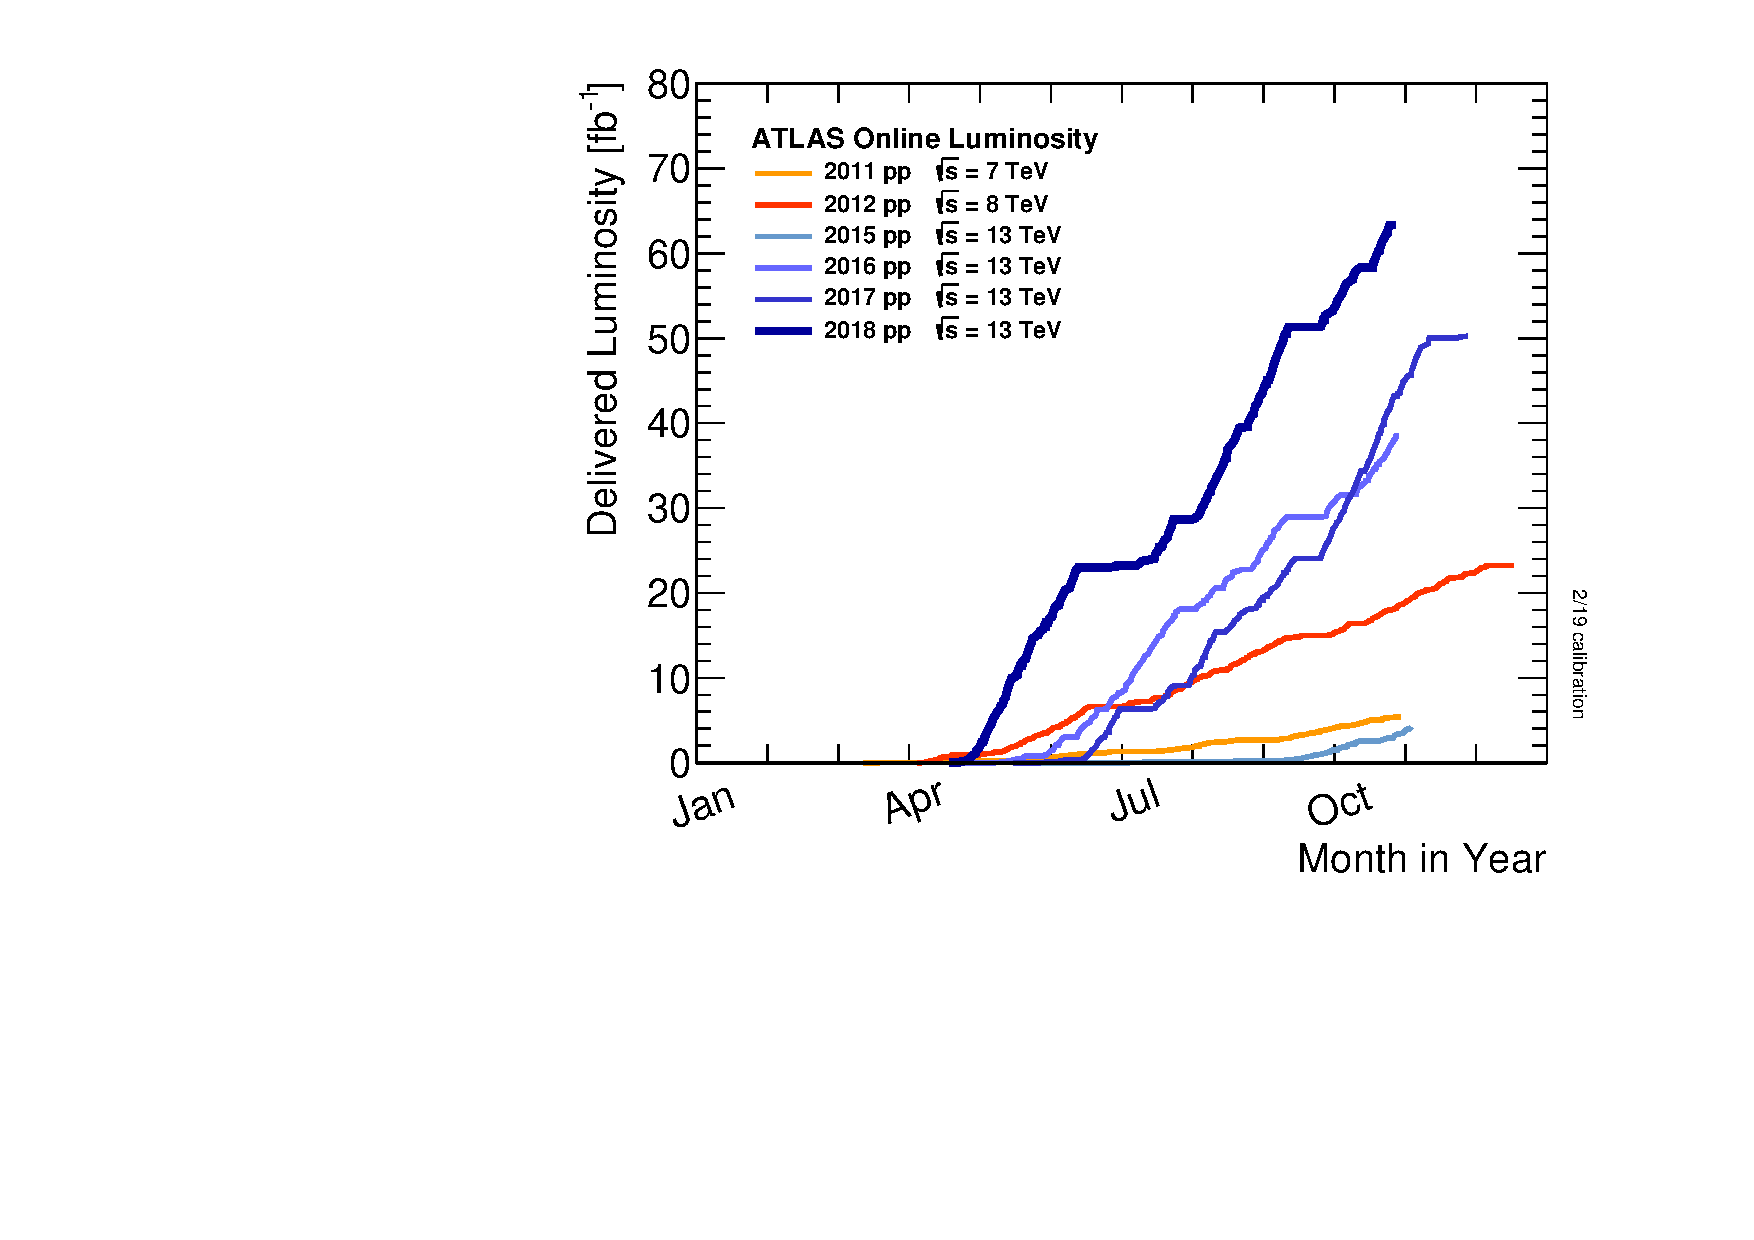
\includegraphics[width=0.5\textwidth]{figures/lhc/intlumivsyear.pdf}}\hfill
\subcaptionbox{2018 Peak Instantaneous Luminosity\label{fig:peakLumiByFill}}{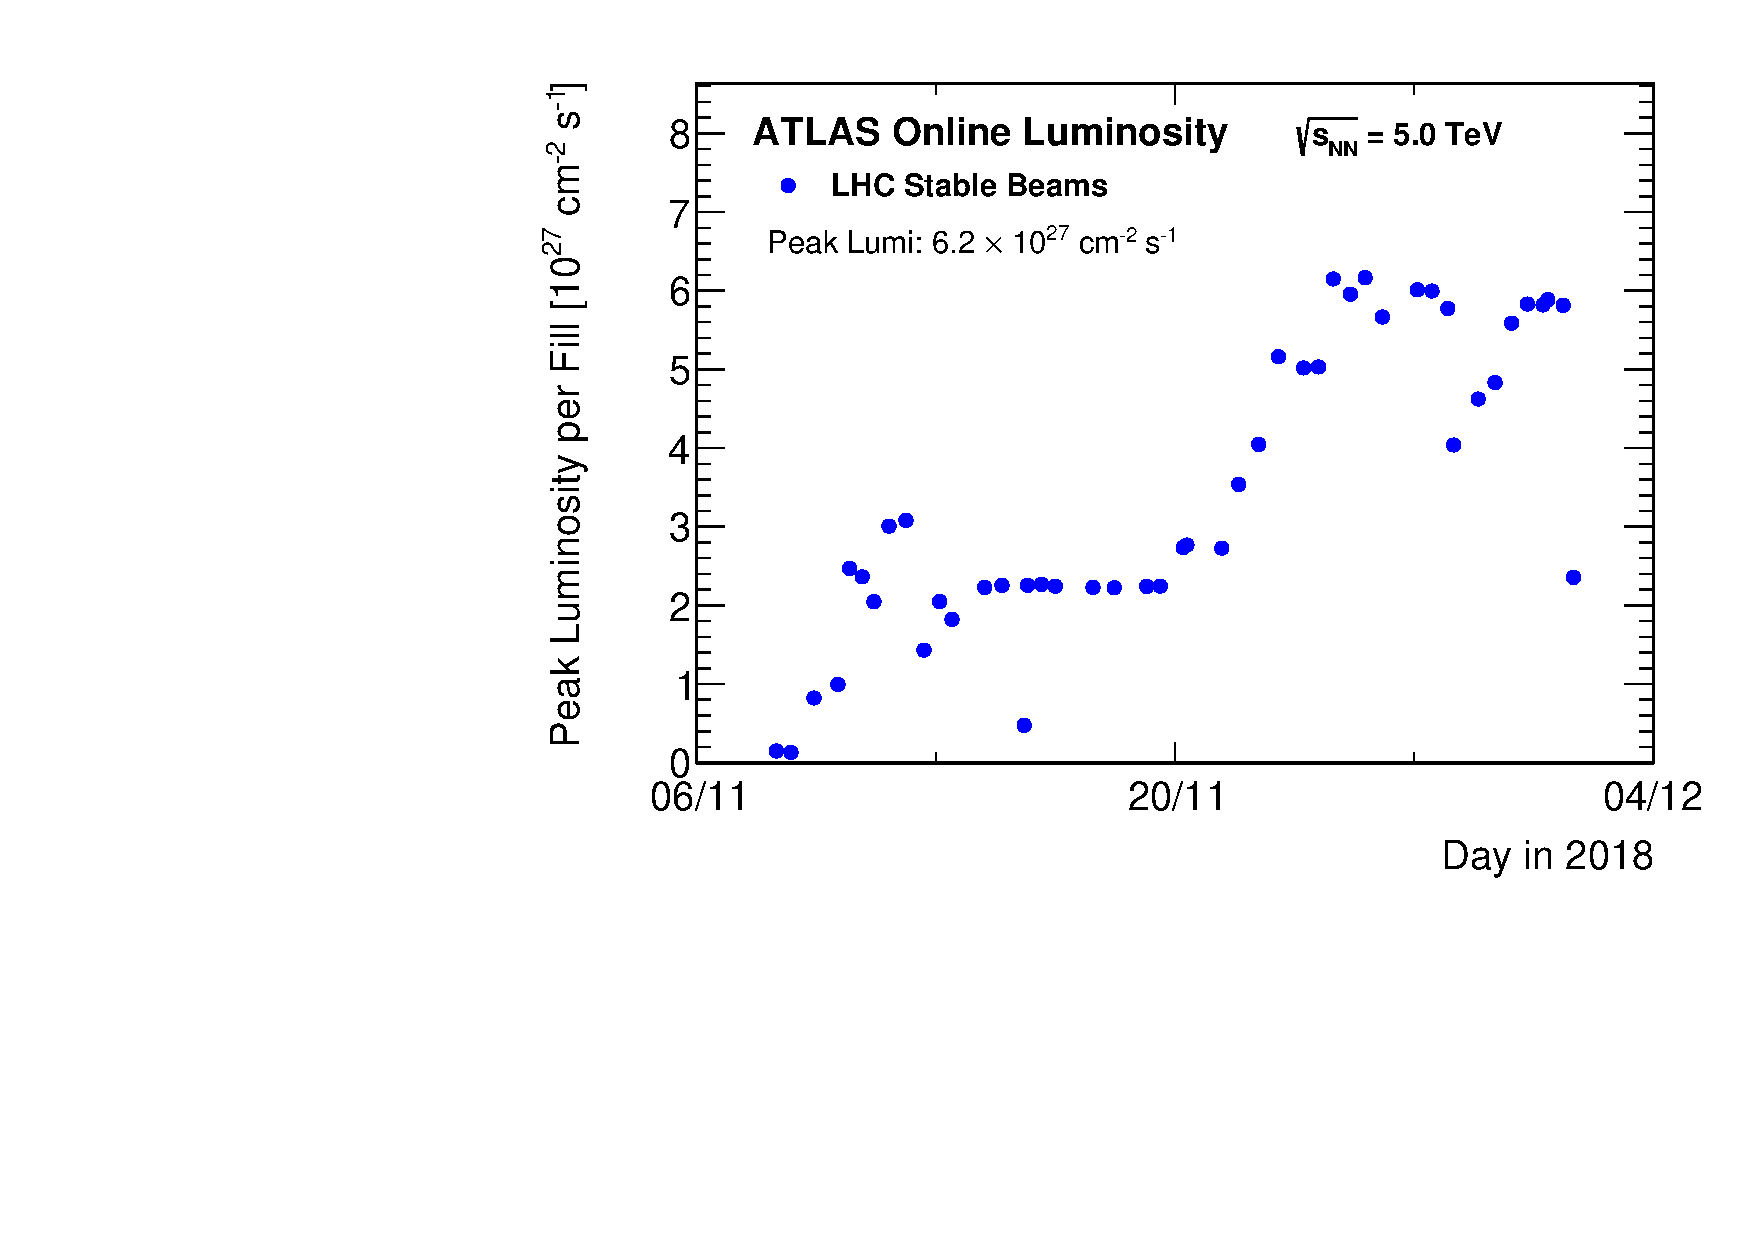
\includegraphics[width=0.5\textwidth]{figures/lhc/peakLumiByFill.pdf}}\hfill
\caption{Luminosity is monitored as both a running total known as the Integrated
Luminosity as depicted in (a) and as an instantaneous quanity as shown in (b).}
\label{fig:luminosity} 
\end{figure}

